\section{Kalman Filter}
\begin{frame}{Problem Formulation}

Recall that the algorithm for Kalman filter is the same for every system. \\~\\

Only need to define state vector $x$, measurement vector $z$, update function $f$, measurement function $h$ and differential matrices $F$ and $H$.


\begin{equation}
    \label{eq:non_linear_update}
    x_{k} = f( x_{k-1}, u_k) + v_k
\end{equation}

\begin{equation}
    \label{eq:non_linear_meas}
    y_k = h (x_k) + w_k
\end{equation}

\begin{equation}
    F = \left. \frac{\partial f(x)}{\partial x} \right\vert_{x = x_{k-1}}; \quad
    H = \left. \frac{\partial h(x)}{\partial x} \right\vert_{x = x_{k}}
\end{equation}

\end{frame}

\begin{frame}{Euler Angles}
\begin{itemize}
\item Euler angles are used as a reference system to measure attitude. \\~\\
\item Tait-Bryan angles are used for navigation purposes. Same as Euler but the reference is different. \\~\\
\item Since we are not using magnetometer, we will just take into account pitch and roll ($\theta$ and $\phi$ resp).
\end{itemize}

\begin{center}
\begin{tabular}{cc}
    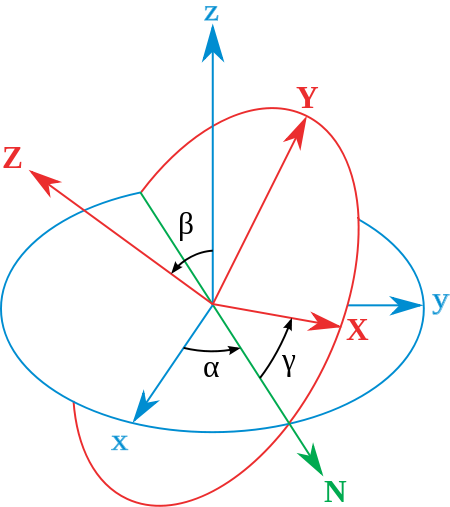
\includegraphics[width=0.25\textwidth]{figures/euler_angles.png} &
    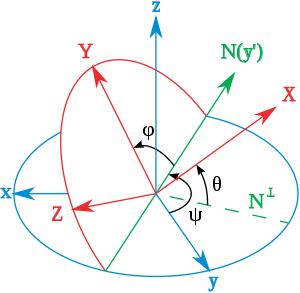
\includegraphics[width=0.25\textwidth]{figures/brian.png}
    \\
    Euler angles & Tait–Bryan angles
\end{tabular}
\end{center}
\end{frame}

\begin{frame}{Problem matrices}
Even though we are not measuring yaw ($\psi$), we still take it to acount in the system states since it does have an impact in giroscopic measures.

\begin{equation}
    x_k = 
        \begin{pmatrix}
            \varphi_k \\
            \theta_k \\
            \psi_k
        \end{pmatrix}
\end{equation}

The accelerometer measurements will be transformed to attitude estimation through a simple transformation:

\begin{equation}
    z =
    \begin{pmatrix}
        \theta\\
        \varphi
    \end{pmatrix}
    = 
    \begin{pmatrix}
        asin \left( \frac{a_x}{g} \right) \\
        asin \left( -\frac{a_y}{g \cos \theta} \right)
    \end{pmatrix}
\end{equation}

For that, the expression of $H$ is very simple:

\begin{equation}
H =
\begin{pmatrix}
1 & 0 & 0 \\
0 & 1 & 0
\end{pmatrix}
\end{equation}

\end{frame}

\begin{frame}{Title}

We need a transformation $T$ between the angular rates from gyroscope and the angular velocities of the fixed frame. 
\begin{itemize}
\item $\dot{\varphi}$, $\dot{\theta}$ and $\dot{\psi}$ are the angular velocities of the fixed frame
\item $p$, $q$ and $r$ are the angular rates from the gyroscopes.
\end{itemize}

\begin{equation}
    \dot{x} =
    \begin{pmatrix}
        \dot{\varphi} \\
        \dot{\theta} \\
        \dot{\psi}
    \end{pmatrix}
    = \begin{pmatrix}
        1 & \sin \varphi \tan \theta & \cos \varphi \tan \theta \\
        0 & \cos \varphi & - \sin \varphi \\
        0 & \frac{\sin \varphi}{\cos \theta}  & \frac{\cos \varphi}{\cos \theta}
    \end{pmatrix}
    \begin{pmatrix}
        p \\
        q \\
        r
    \end{pmatrix}
\end{equation} 

Now the update function can be defined as:

\begin{equation}
f(x,p,q,r,dt) = x + T
\begin{pmatrix}
p \\ q \\ r
\end{pmatrix}
dt = x + \dot{x} dt
\end{equation}

\end{frame}


\begin{frame}{Problem matrices}
The differencial matrix is a bit trickier, since the derivatives are with respect to the euler angles and not the angle rates.

\fontsize{9pt}{10pt}\selectfont
\begin{equation}
   F = I + dt
   \begin{pmatrix}
       q \cos\varphi \tan\theta - r \sin\varphi \tan \theta &
       q \sin \varphi \sec^2 \theta + r \cos \varphi \sec^2 \theta &
       0 \\
       -q \sin \varphi - r \cos \varphi
       & 0 & 0 \\
       q \cos \varphi \sec \theta - r \sin \varphi \sec \theta &
       q \sin \varphi \sec \theta \tan \theta + r \cos\varphi \sec \theta \tan  \theta &
       0
   \end{pmatrix}
\end{equation}


\end{frame}


\begin{frame}{Kalman Filter}
\begin{equation}
\begin{array}{c}
    \hat{x}_k = f(x_{k-1},p,q,r,dt) \\
    \hat{P_k} = F_k P F_k' + Q \\
    K_k = \hat{P_k} H \left(H \hat{P_k} H' + R\right)^{-1} \\
    x_k = \hat{x}_k + K_k \left(z_k - H \hat{x}_k \right) \\
    P_k = \hat{P}_k - K H \hat{P}_k 
\end{array}
\end{equation}
\end{frame}